
\chapter{Fine-Tuning And Results \label{Chapter_Evaluation}}

Fine-Tune is an approach to transfer learning where we update the weights of pre-trained model according to the new data. Usually models that are pre-trained on large corpora are fine-tuned by reusing the model's parameters as a initial point and a task-specific layer such as relation extraction, named entity recognition, question answers, semantic analysis, token classification and so on is added which can be trained from the scratch or partially. Fine-tuning can be achieved on entire neural network or a subset of that, where remaining layers from this subset is known as "frozen layers" (layers is not updated in backpropagation process). Fine-tuning is generally achieved in supervised learning manner, however there are few techniques to fine-tune a model using weak supervision \cite{yu2020fine}.

\section{Comparison of LiLT on Semantic Entity Recognition}
 As we discussed in \Cref{datasets} that \acrshort{lilt} can be pre-trained with monolingual and multi-lingual text based models, which can be fine-tune further on specific tasks and language. \acrshort{lilt} has been used with different text based models in order to process the text in a document for text flow and different datasets and languages in those datasets leads to vary the performance of LiLT when its being combined with various text based models for the same task(\acrshort{ser}). For instance, when LiLT is combined with RoBERTa\(_{BASE}\) (LiLT[EN-R]\(_{BASE}\)), which is a text based model pre-trained on English language dataset. During the fine-tunnig for \acrfull{ser} it shows different F1 scores, the comparison of LiLT[EN-R]\(_{BASE}\) over different datasets is shown in \Cref{tab:compare_dataset_f1_english}. We can see the model LiLT[EN-R]\(_{BASE}\) which is pre-trained on English dataset and fine-tuned in Indonesian language have higher F1 than the one fine-tuned in English. In \Cref{tab:compare_datasets_f1_multilingual}, the fine-tuning results of LiLT[InfoXLM]\(_{BASE}\) for \acrshort{ser} task using different datasets and language is shown,  which uses InfoXLM\(_{BASE}\) a pre-trained text-based model pre-trained on multi-lingual corpus for text flow.  The use of multi-lingual text-based model (LiLT[InfoXLM]\(_{BASE}\)) in combination with LiLT shows slighly less performance with compare to combination of LiLT with monolingual text-based models (LiLT[EN-R]\(_{BASE}\)) on \acrshort{ser} when its being fine-tuned in one specific language. 

 \begin{table}[!ht]
     \centering
     \begin{tabular}{lcl}
     \toprule
     \textbf{Dataset} &\textbf{Language for fine-tuning} &\textbf{F1} \\ \midrule
          FUNSD& English& 0.884 \\
          CORD& Indonesian &0.960 \\ \bottomrule
     \end{tabular}
     \caption{Fine-tuning results of LiLT[EN-R]\(_{BASE}\) on different language for \acrshort{ser} task}
     \label{tab:compare_dataset_f1_english}
 \end{table}

\begin{table}[!ht]
    \centering
    \begin{tabular}{lcl}
    \toprule
    \textbf{Dataset}&\textbf{Language for fine-tuning}& \textbf{F1}\\ \midrule
         FUNSD& English&0.85  \\
         CORD& Indonesian & 0.957\\
         XFUND& Deutsch & 0.823 \\ \bottomrule
    \end{tabular}
    \caption{Fine-tuning results of LiLT[InfoXLM]\(_{BASE}\) on different language \acrshort{ser} task}
    \label{tab:compare_datasets_f1_multilingual}
\end{table}


\section{Comparison of LiLT on Token Classification}
Document content classification or text classification, also known as token classification is a slightly different task than \acrshort{ser}. Instead of classifying document content into specific classes like person's name, location, dates, quantieties and so on, token classification refers to classifying content into broad and general sections such as question, header, answer and so on. In previous sections, we explored LiLT in combinations with different types of text based models and different datasets with different language for \acrshort{ser} task. However,  to the best of our knowledge, there is only one text-based model in combination with LiLT available that is fine-tuned for \acrshort{ser} task for German language documents. The LiLT[InfoXLM]\(_{BASE}\) fine-tuned by \cite{wang-etal-2022-lilt} over XFUND dataset over different languages for \acrshort{ser} that includes total 7 languages including German(\Cref{tab:Comparision_Xfund}). In addition, most experiments on \acrshort{lilt} has been done over \acrshort{ser} tasks and there are very few experiments available that shows the performance of \acrshort{lilt} over document content or text classification. For instance, the GitHub repository \footnote{\url{https://github.com/NielsRogge/Transformers-Tutorials/tree/master/LiLT}, Accessed: 15.04.2024 \label{fine-tune-token-classification}} contains information on combining the \acrshort{lilt} with different text-based models, fine-tune the combined models or available base models provided by \cite{wang-etal-2022-lilt} over FUNSD or custom datasets. In \Cref{tab:Compare_FUNSD_token_classification}, the comparison between different combinations of \acrshort{lilt} with text-based models, datasets, epoch and F1 on token classification task is described from GitHub repository\(^{\ref{fine-tune-token-classification}}\). An epoch refers to one cycle of training the model over complete train-dataset. 

\begin{table}[!ht]
    \centering
    \captionsetup{justification=centering}
    \begin{tabular}{lcccl}
    \toprule
    \textbf{Model}& \textbf{Dataset}& \textbf{Language} & \textbf{Epoch} &\textbf{F1}\\ \midrule
     \(\text{LiLT[XLM-RoBERTa]}_{BASE}\)& FUNSD & English & 20 & 0.735 \\
     \(\text{LiLT[EN-R]}_{BASE}\) & FUNSD & English & 50 & 0.771 \\
     \(\text{LiLT[EN-R]}_{BASE}\)& FUNSD & English & 106 & 0.806 \\ \bottomrule
    \end{tabular}
    \caption{Comparison of fine-tuning results of LiLT with different text-based models  on FUNSD for token classification task available on GitHub repository\(^{\ref{fine-tune-token-classification}}\) }
    \label{tab:Compare_FUNSD_token_classification}
\end{table}


By looking at the fine-tune results of \acrshort{lilt} in combination with mono-lingual and multi-lingual text based models for \acrshort{ser} and token classification tasks on an English language dataset FUNSD, it is clear that the combination of \acrshort{lilt} with mono-lingual text based model (\(\text{LiLT[EN-R]}_{BASE}\)) shows highet F1 in both token classification and \acrshort{ser} tasks. Therefore, in our work we will try to find out the performance of \acrshort{lilt} in combination with monolingual and multi-lingual text-based pre-trained models on token classification task for German language. This will help to choose the best model that is performing good for German language documents and still can be used for multi-lingual documents on token classification task.    








\section{Fine-Tuning LiLT}

As we discussed in above, when we use the \(\text{LiLT[EN-R]}_{BASE}\), which is a combination of \acrshort{lilt} with text-based model pre-trained on English language dataset, it shows higher F1 after fine-tuning for \acrfull{ser} task with compare to the model \(\text{LiLT[info-XLM]}_{BASE}\) which is a combination of \acrshort{lilt} with text-based model pre-trained on multi-lingual dataset (Please refer to \Cref{tab:compare_dataset_f1_english} and \Cref{tab:compare_datasets_f1_multilingual}). We also discussed the fine-tunning performance of both models on token classification task using English language dataset (\Cref{tab:Compare_FUNSD_token_classification}). However, all the results mentioned in above are mostly based on English language datasets, there is only one model (\(\text{LiLT[info-XLM]}_{BASE}\)) results available for \acrshort{ser} task that is fine-tuned using documents in German language (\Cref{tab:compare_datasets_f1_multilingual}). Therefore, we will combine the \acrshort{lilt} with different mono-lingual and multi-lingual text-based model to evaluate the model performance on token classification task on German language documents to find the suitable model for deployment. 


\subsection{Fine-tuning results for 30 epoch}
We have used text-besed models like RoBERTa and XLM-RoBERTa in order to combine it with \acrshort{lilt}. RoBERTa is a text-based model that has been pre-trained on English language dataset and XLM-RoBERTa is pre-trained on multi-lingual dataset. We started with 30 epoch to see the results of these models in combination with \acrshort{lilt} on German language dataset for token classification task since the fine-tuning of these model takes large amount of computing resources. The fine-tuning results of \acrshort{lilt} for 30 epoch with different combination of text-based model over German language dataset for token classification task is shown in \Cref{tab:30_epoch_results}. In this setting, the mono-lingual text-based models in combination with \acrshort{lilt} shows higher overall scores with compare to multi-lingual text-based model. The classification results of \(\text{LiLT[En-R]}_{BASE}\) on all classes(\ref{multi_class}) is described in \Cref{fig:multi_calss_en_lilt}, The model performance on classes \verb|HEADER, QUESTION, ANSWER|  are described in \Cref{Listing:main_Classes_res_30_epoch}. However, in table, we saw \(\text{LiLT[InfoXLM]}_{BASE}\) shows overall f1 of 0.823 for \acrshort{ser} task on German language dataset. Therefore, we also include  \(\text{LiLT[InfoXLM]}_{BASE}\) for token classification task on German language dataset to compare the fine-tune results between two multi-lingual text-based models. We can see that the model pre-trained on multi-lingual dataset (XLM-RoBERTa and InfoXLM) shows nearly identical results. 

\begin{table}[!ht]
    \centering
    \captionsetup{justification=centering}
    \begin{tabular}{lcccl}
        \toprule
        \textbf{Model}& \textbf{Precision}& \textbf{Recall}& \textbf{F1} & \textbf{Accuracy}\\ \midrule
        \(\text{LiLT[InfoXLM]}_{BASE}\)& 0.378& 0.537& 0.444& 0.636 \\ \midrule
         \(\text{LiLT[En-R]}_{BASE}\) &  0.744& 0.795& 0.768& 0.756 \\
         \(\text{LiLT[XLM-RoBERTa]}_{BASE}\)& 0.359& 0.535& 0.430& 0.627 \\ \bottomrule
    \end{tabular}
    \caption{Fine-tuning results of \acrshort{lilt} in combination with different text-based models on German language dataset for token classification task over 30 epoch}
    \label{tab:30_epoch_results}
\end{table}

\begin{listing}[!ht]

\begin{minted}{python}
{
0: 'O', 
1: 'B-HEADER', 
2: 'I-HEADER', 
3: 'B-QUESTION', 
4: 'I-QUESTION', 
5: 'B-ANSWER', 
6: 'I-ANSWER'
}
\end{minted}
\caption{Labels(Classes) Assigned to number}
\label{multi_class}
\end{listing}


\begin{listing}[!ht]
\captionsetup{justification=centering}
\begin{minted}{python}
    'ANSWER':  {'precision': 0.78515625, 'recall': 0.7905604719764012,
                'f1': 0.7878490935815776, 'number': 1017},
    'HEADER':  {'precision': 0.6, 'recall': 0.46551724137931033,
                'f1': 0.5242718446601942, 'number': 58},
    'QUESTION':{'precision': 0.7019464720194647, 'recall': 0.8290229885057471,
                'f1': 0.7602108036890646, 'number': 696}
\end{minted}
\caption{Results on Classes \(\text{LiLT[En-R]}_{BASE}\)(\Cref{tab:30_epoch_results}), \\ fine-tuned-language: German, Evaluation-dataset-language:German }
\label{Listing:main_Classes_res_30_epoch}
\end{listing}

\begin{figure}[!ht]
    \centering
    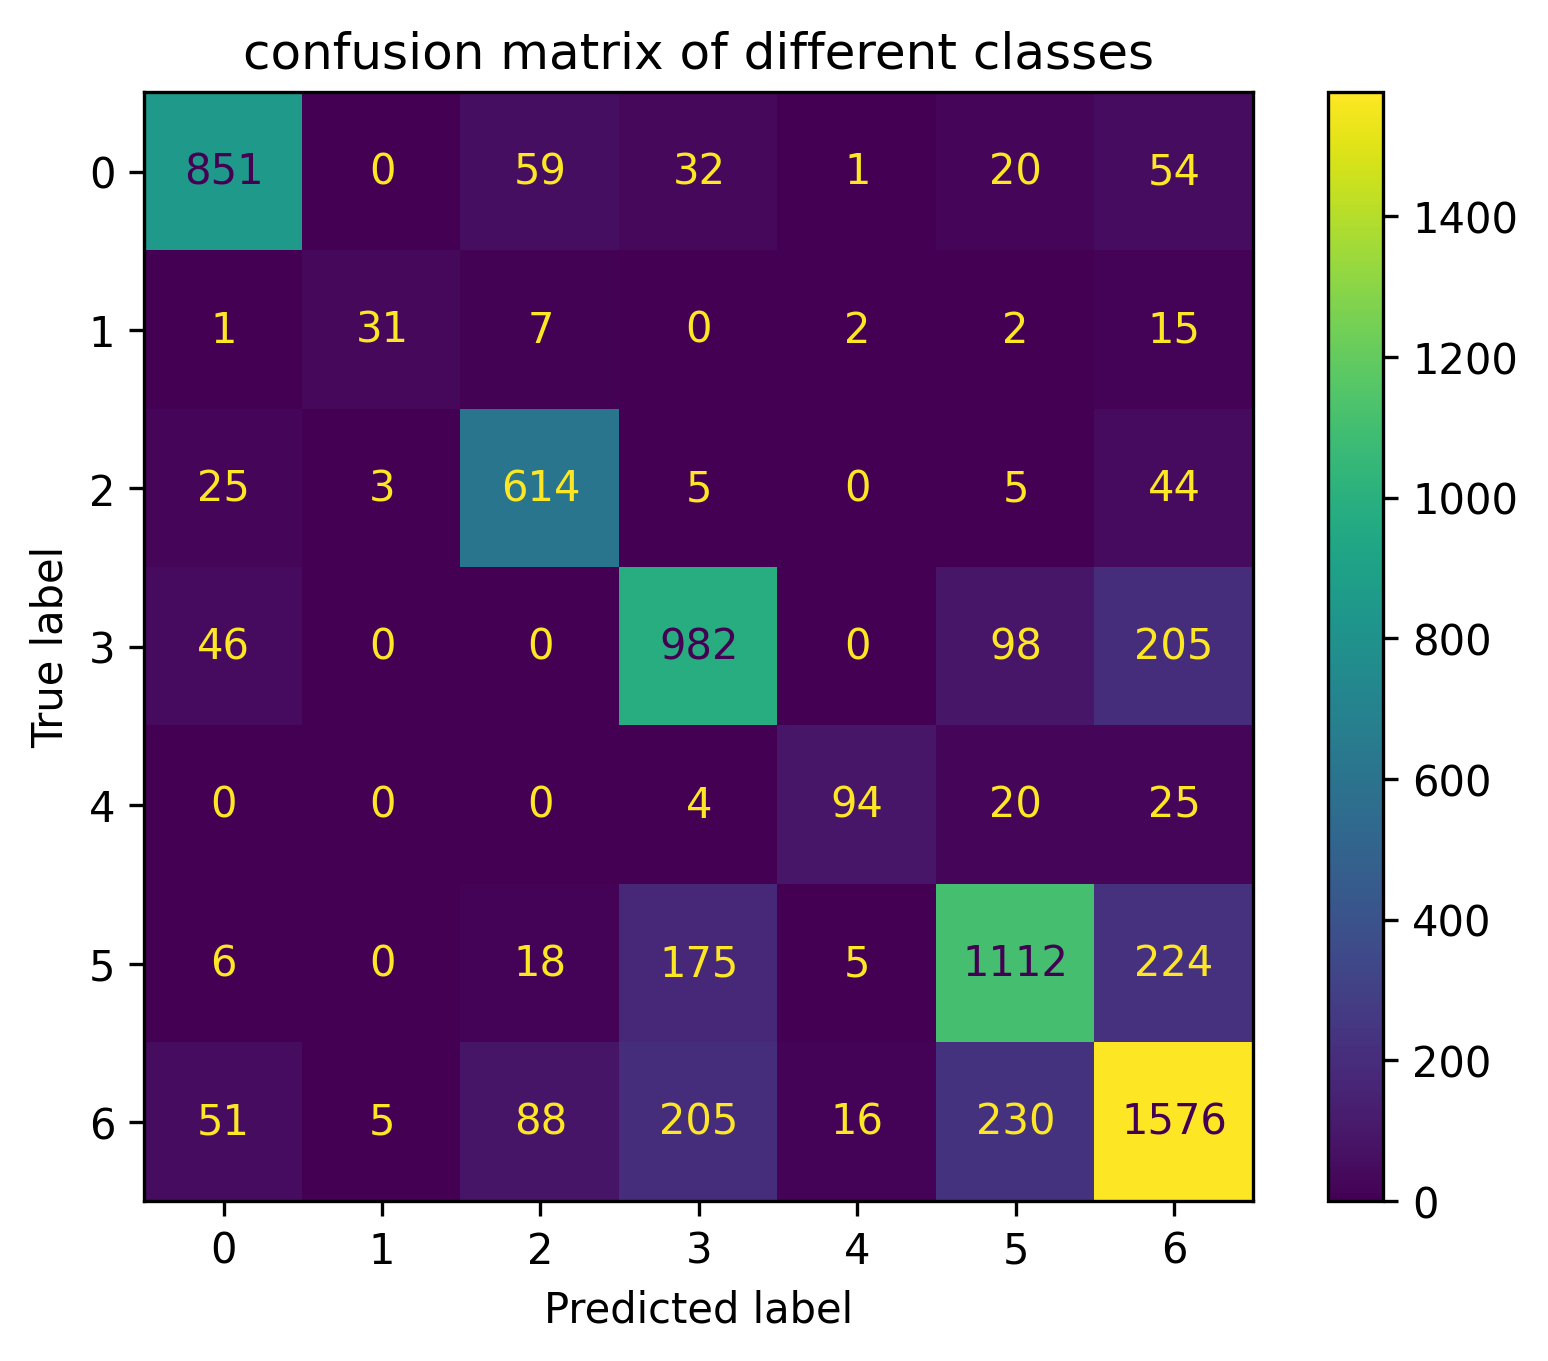
\includegraphics[width=0.6 \textwidth]{chapters/images/experiments_and_results/En_LiLT_30_output.png}
    \caption{Confusion matrix of all classes using \(\text{LiLT[En-R]}_{BASE}\) from \Cref{tab:30_epoch_results} }
    \label{fig:multi_calss_en_lilt}
\end{figure}
    
% \begin{figure}[H]
%     \centering
%     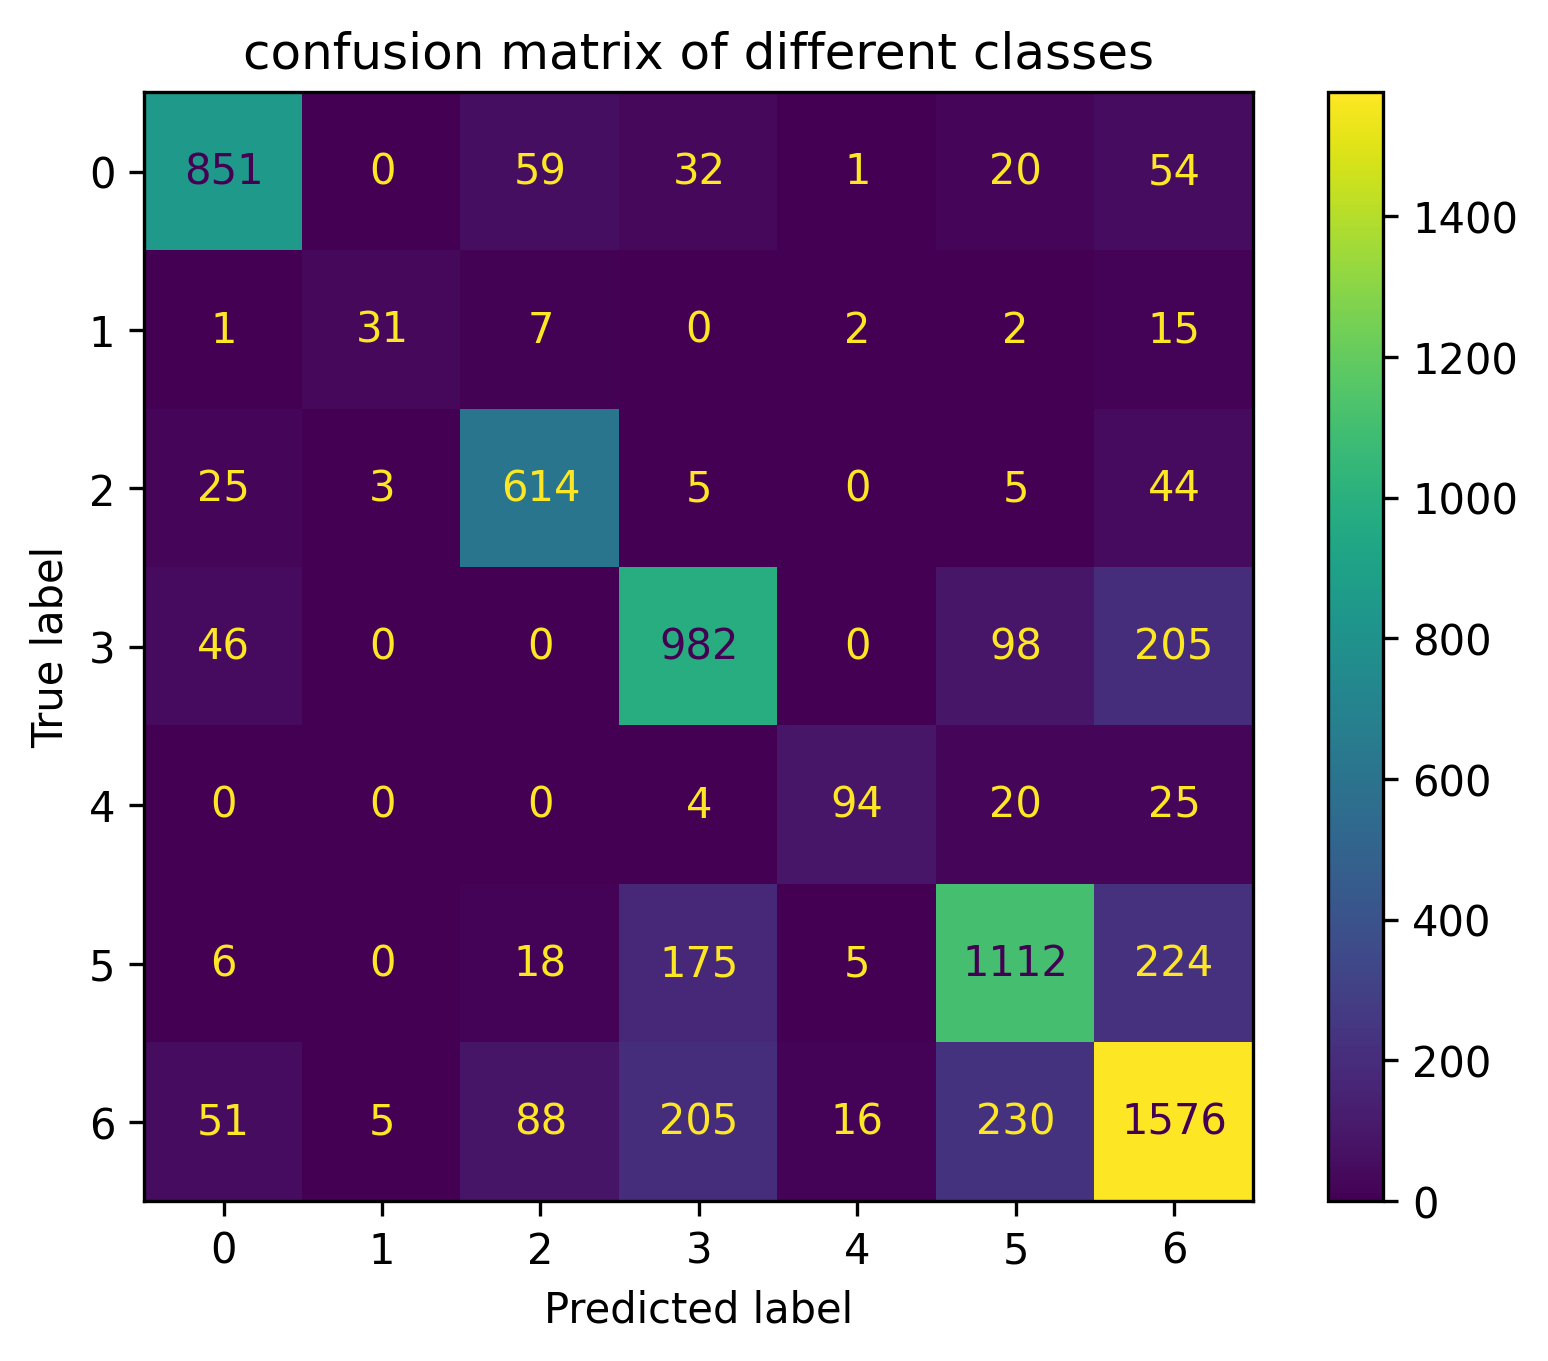
\includegraphics[width=0.6 \textwidth]{chapters/images/experiments_and_results/En_LiLT_30_output.png}
%     \caption{Confusion matrix of all classes using \(\text{LiLT[En-R]}_{BASE}\) from \Cref{tab:30_epoch_results} }
%     \label{fig:multi_calss_en_lilt}
% \end{figure}





\subsection{Fine-tuning result of LiLT for 100 epoch}
Due to the high demand of resource and computing power needed to fine-tune these models for 100 epoch, it is time consuming and costly to fine-tune all the models over large number of training cycles. For instance, it took almost 2 and a half day to fine-tune \(\text{LiLT[XLM-RoBERTa]}_{BASE}\) using Intel Core i7-1185G7 Processor\footnote{\url{https://www.intel.com/content/www/us/en/products/details/processors/core.html}, Accessed: 3.5.2024}. If we want to use the same settings and fine-tune the model using AWS EC2, It would cost around \$ 30 for each training using models in the BASE settings. However, as the size of the model rises, the cost rises dramatically making it a key concern to choose right resources and methods to choose to cut down the cost before the training. According to the \Cref{tab:Compare_FUNSD_token_classification}, for English language dataset, LiLT[XLM-RoBERTa] achieves F1 score of 0.735 within 20 epoch, where the same model shows 0.430 F1 for German language dataset on token classification within 30 epoch(\Cref{tab:30_epoch_results}). Moreover, LiLT[EN-R] reaches 0.771 F1 for 50 epoch and the highest 0.806 over 106 epoch, on other hand the same model for German language dataset reached 0.76 F1 within 30 epoch(\Cref{tab:30_epoch_results}). The combination of English-RoBERTa shows good performance in both the dataset (English and German) within less number of epochs. Since InfoXLM and XLM-RoBERTa are pre-trained on multi-lingual dataset and both shows almost similar performance for 30 epoch, therefore we kept one type of model (RoBERTa) for large amount of training to save time and cost over computing resources. We fine-tuned LiLT[XLM-RoBERTa] and LiLT[EN-R] for 100 epoch on German language dataset for token classification task and achieved 0.707 F1 for LiLT[XLM-RoBERTa] and LiLT[EN-R] overall F1 was 0.763, The results of the metric are shown in \Cref{tab:100_epoch_results}. In \Cref{fig:Multi-class_XLM}, the confusion matrix for all classes is described for LiLT[XLM-RoBERTa],  LiLT[EN-R] fine-tuned with 30 epochs shows better results than with 100 epochs, the confusion matrix for different classes and overall results for LiLT[EN-R] is described in \Cref{fig:multi_calss_en_lilt} and \Cref{tab:30_epoch_results}. In \Cref{fig:Multi-class_XLM}, the numbers in axis represents the labels as shown in \Cref{multi_class}.


\begin{table}[!ht]
    \centering
    \captionsetup{justification=centering}
    \begin{tabular}{lcccl}
        \toprule
        \textbf{Model}& \textbf{Precision}& \textbf{Recall}& \textbf{F1} & \textbf{Accuracy}\\ \midrule
         \(\text{LiLT[En-R]}_{BASE}\) &  0.743& 0.783& 0.763& 0.752 \\
         \(\text{LiLT[XLM-RoBERTa]}_{BASE}\)& 0.686& 0.728& 0.707& 0.757 \\ \midrule
    \end{tabular}
    \caption{Fine-tuning results of \acrshort{lilt} in combination with different text-based models on German language dataset for token classification task over 100 epoch}
    \label{tab:100_epoch_results}
\end{table}



\begin{figure}[!ht]
    \centering
    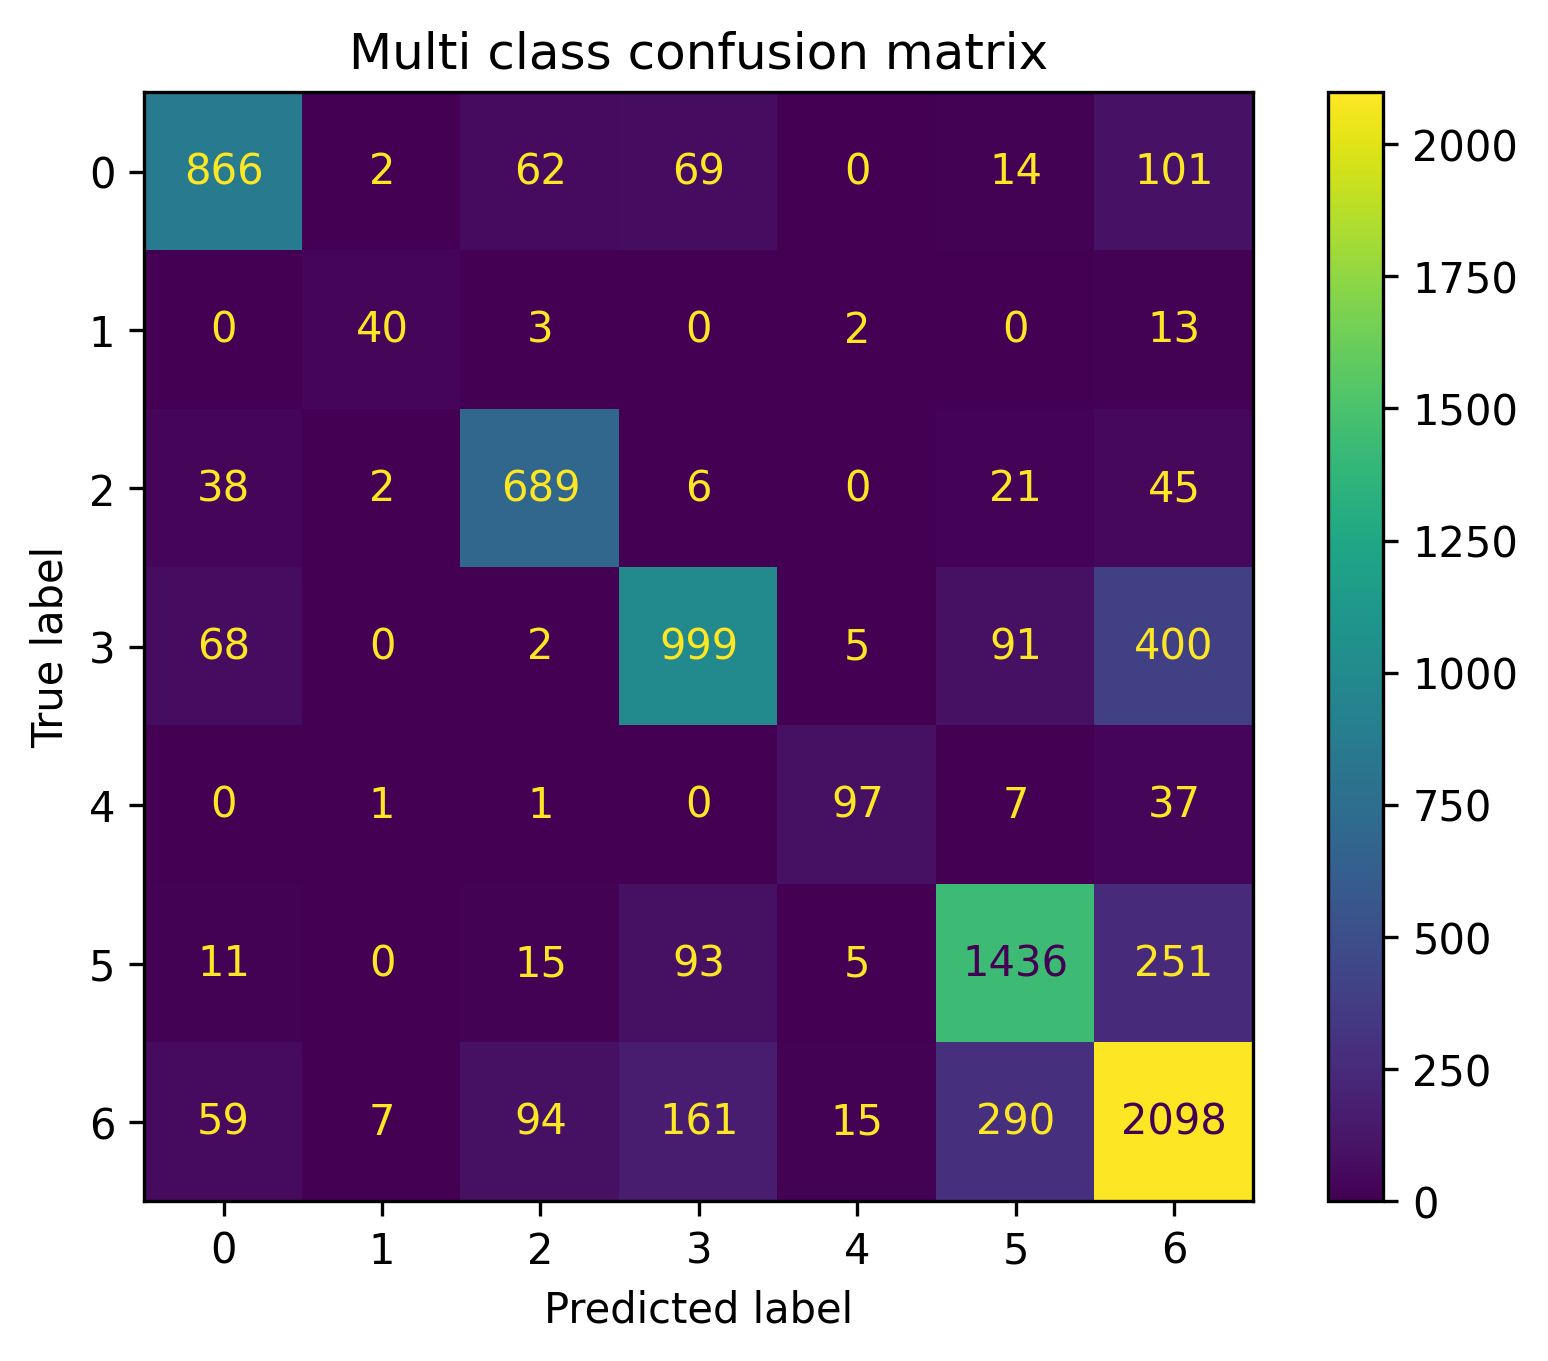
\includegraphics[width=0.6 \textwidth]{chapters/images/experiments_and_results/XLM_100_output.png}
    \caption{Confusion matrix of all classes(\ref{multi_class}) using \(\text{LiLT[XLM-RoBEERTa]}_{BASE}\) from \Cref{tab:100_epoch_results}}
    \label{fig:Multi-class_XLM}
\end{figure} 

\subsection{Results of Fine-tuned LiLT in German language with other Languages}
Pre-training and Fine-tunning are crucial steps in \acrshort{nlp}, during the pre-training, the model learns about linguistic structures, grammar and semantic understanding at some level. As we discussed \acrshort{lilt} can be used in combination with text-based models like RoBERTa and XLM-RoBERTa, where RoBERTa is pre-trained using English language and XLM-RoBERTa is pre-trained using around 100 languages. While in fine-tuning on specific task such as token classification, model adapt its general knowledge from pre-traing to the spcific tasks. The combinations of pre-trained \acrshort{lilt} with EN-RoBERTa and XLM-RoBERTa are available at GitHub\footnote{\url{https://huggingface.co/nielsr}, Accessed: 03.05.2024 \label{base_models}} that are pre-trained using FUNSD dataset which is an English language dataset. As we discussed above, We used LiLT[EN-R] and LiLT[XLM-RoBERTa] and fine-tuned for token classification task using German language dataset, the model shows good results on German language datasets since its been fine-tuned on German language and weights are adapted to that language. At this point, both model's weights are first changed while pre-training using FUNSD and fine-tuning using German language dataset. In addition, during fine-tuning the layout information is also being added to the model's knowledge. We have used XFUND dataset that is having 7 languages to compare the results of LiLT[XLM-RoBERTa] pre-trained on FUNSD and LiLT[XLM-RoBERTa] fine-tuned on token classification task using German language dataset. Since, the XFUND dataset was missing features like "\verb|words|" of the documents, instead XFUND comes with "\verb|input_ids|" feature and using multi-lingual tokenizer for LiLT[EN-R] was not possible. Therefore, LiLT[EN-R] was excluded from the evaluation for XFUND dataset except German since there is a German language subset of XFUND avaialable at Hugging face hub\footnote{\url{https://huggingface.co/datasets/cooleel/xfund_de}, Accessed: 05.05.2024} that have features like \verb|words| of each documents and therfore there was a possibility to include LiLT[EN-R] for German and English language. In table, the evaluation results of fine-tuned LiLT[EN-R] in German language for token classification task is shown in \Cref{tab:EN_R_on_different_languages} and the evaluation results of LiLT[XLM-RoBERTa] on different languages are described in \Cref{tab:Eval_on_different_language}. 


\begin{listing}[!ht]

\begin{minted}{python}
            { FR: 'French', ES: 'Spanish', IT: 'Italian', PT: 'Portuguese', 
            JA: 'Japanese', ZH: 'Chiense', DE: 'German', EN: 'English' }
\end{minted}
\caption{Languages}
\label{languages}
\end{listing}


\begin{table}[!ht]
    \centering
    \captionsetup{justification=centering}
    \begin{tabular}{lccccl}
        \toprule
         \textbf{Dataset}& \textbf{Language}& \textbf{Precision}& \textbf{Recall}& \textbf{F1} & \textbf{Accuracy}  \\ \midrule
         FUNSD & EN & 0.52641 & 0.41082 & 0.46149 & 0.54629\\
         XFUND & DE &  0.74457 & 0.79503 & 0.76897 & 0.75618 \\ \bottomrule
    \end{tabular}
    \caption{Comparison of fine-tuned LiLT[EN-R] using German language documents with different languages(\cref{languages})}
    \label{tab:EN_R_on_different_languages}
\end{table}


\begin{table}[!ht]
    \centering
    \captionsetup{justification=centering}
    \begin{tabular}{lccccl}
    \toprule
    \textbf{Dataset}& \textbf{Language} & \textbf{Precision} &\textbf{Recall} & \textbf{F1} & \textbf{Accuracy}\\ \midrule
    \multirow{7}{*}{XFUND} &FR  &0.00392  & 0.00952 &0.00555  &0.24706 \\
                  &  ES&0.00279  &0.00724  &0.00403  &0.21296  \\
                  & IT& 0.00478 & 0.01193 & 0.00683 & 0.19410\\
                  & PT & 0.00429 & 0.00885 & 0.00578 & 0.20010\\
                  & JA & 0.00324 & 0.00766 & 0.00455 & 0.29468 \\
                  & ZH & 0.00456 & 0.00821 & 0.00586 & 0.18616\\
                  &DE & 0.68672& 0.72715&  0.70715& 0.75766 \\  \midrule
                FUNSD  & EN& 0.37032 & 0.32297 & 0.34503 & 0.49394\\ \bottomrule
                  
    % \multirow{2}{*}{FUNSD} & \(\text{EN}_{\text{LiLT[EN-R]}}\) & 0.52641 & 0.41082 & 0.46149 & 0.54629\\
    %                         & EN& 0.37032 & 0.32297 & 0.34503 & 0.49394\\ \midrule
    % \multirow{2}{*}{XFUND} & \(\text{DE}_{\text{LiLT[EN-R]}}\) & 0.74457 & 0.79503 & 0.76897 & 0.75618 \\
                                
    \end{tabular}
    \caption{Comparison of fine-tuned LiLT[XLM-RoBERTa] using German language documents with different languages(\cref{languages})}
    \label{tab:Eval_on_different_language}
\end{table}